
% ============================================================
%  ENTREGABLE 1 GTI — CO LOGISTIC S.A.C.
%  Compilar: xelatex → xelatex
% ============================================================

\documentclass[11pt, a4paper, oneside]{report}

% ── Fuentes y codificación ───────────────────────────────
\usepackage{fontenc}
\usepackage{babel}
\babelprovide[import, main]{spanish}

% ── Márgenes ────────────────────────────────────────────
\usepackage{geometry}
\geometry{
  top    = 2.54cm,
  bottom = 2.54cm,
  left   = 3.00cm,
  right  = 2.54cm,
}
\setlength{\headheight}{14.5pt}

% ── Interlineado y párrafo ───────────────────────────────
\usepackage{setspace}
\setstretch{1.5}
\usepackage{parskip}
\setlength{\parindent}{1.25cm}

% ── Paquetes generales ───────────────────────────────────
\usepackage{float}
\usepackage{pdflscape}
\usepackage{lscape}
\usepackage{tikz}
\usepackage{graphicx}
\usepackage{chngcntr}
\usepackage{booktabs}
\usepackage{tabularx}
\usepackage{array}
\usepackage{longtable}
\usepackage{enumitem}
\usepackage{caption}
\usepackage{microtype}
\usepackage{amsmath}
\usepackage{ragged2e}
\usepackage{hyperref}
\usepackage{tocloft}

% ── Colores UPeU ────────────────────────────────────────
\usepackage[table]{xcolor}
\definecolor{upeu_dark}{HTML}{1A3A6B}
\definecolor{upeu_mid}{HTML}{2E75B6}
\definecolor{upeu_light}{HTML}{D6E4F0}
\definecolor{upeu_gold}{HTML}{B8860B}
\definecolor{body_gray}{HTML}{404040}
\definecolor{hint_gray}{HTML}{9E9E9E}

% ── Encabezado y pie ────────────────────────────────────
\usepackage{fancyhdr}
\pagestyle{fancy}
\fancyhf{}
\fancyhead[R]{%
  {\color{upeu_dark}\small\bfseries Ingeniería de Sistemas · UPeU}%
}
\renewcommand{\headrule}{{\color{upeu_mid}\rule{\headwidth}{0.8pt}}}
\fancyfoot[L]{{\color{hint_gray}\small\itshape Ingeniería de Sistemas}}
\fancyfoot[R]{{\color{body_gray}\small Página \thepage}}
\renewcommand{\footrule}{{\color{upeu_mid}\rule{\headwidth}{0.8pt}}}

\makeatletter
\let\ps@plain\ps@fancy
\makeatother

% ── Títulos / secciones ──────────────────────────────────
\usepackage{titlesec}

\titleformat{\chapter}[display]
  {\thispagestyle{empty}\normalfont\centering\vspace*{\fill}}
  {\color{upeu_mid}\bfseries\fontsize{20}{30}\selectfont CAPÍTULO \thechapter}
  {0.05cm}
  {\color{upeu_dark}\bfseries\fontsize{30}{40}\selectfont}
  [\vspace*{\fill}\newpage]

\titlespacing{\chapter}{0pt}{0pt}{0pt}

\titleformat{\section}[hang]
  {\normalfont\bfseries\large\color{upeu_dark}}
  {\thesection}{0.7em}{}
\titlespacing{\section}{0pt}{14pt}{6pt}

\titleformat{\subsection}[hang]
  {\normalfont\bfseries\normalsize\color{upeu_mid}\itshape}
  {\thesubsection}{0.7em}{}
\titlespacing{\subsection}{0pt}{10pt}{4pt}

\titleformat{\subsubsection}[hang]
  {\normalfont\bfseries\normalsize\color{body_gray}}
  {\thesubsubsection}{0.7em}{}
\titlespacing{\subsubsection}{0pt}{8pt}{2pt}

\setcounter{secnumdepth}{3}
\setcounter{tocdepth}{3}

% ── Índice ───────────────────────────────────────────────
\renewcommand{\cfttoctitlefont}{\normalfont\bfseries\Large\color{upeu_dark}}
\setlength{\cftbeforetoctitleskip}{10pt}
\setlength{\cftaftertoctitleskip}{16pt}
\renewcommand{\cftchapfont}{\bfseries\color{upeu_dark}}
\renewcommand{\cftsecfont}{\color{body_gray}}
\renewcommand{\cftsubsecfont}{\small\color{body_gray}}
\renewcommand{\cftchapleader}{\cftdotfill{\cftdotsep}}
\renewcommand{\cftsecleader}{\cftdotfill{\cftdotsep}}

% ── Imágenes ─────────────────────────────────────────────
\graphicspath{{./img/}}
\counterwithout{figure}{chapter}
\counterwithout{table}{chapter}

\newcommand{\figura}[3][0.85\linewidth]{%
\begin{figure}[H]
\centering
\IfFileExists{img/#2}{%
  \includegraphics[width=#1]{#2}%
}{%
  \fbox{%
    \begin{minipage}[c][4.5cm][c]{#1}
    \centering
    \small Imagen pendiente: \texttt{#2}\\
    Subir este archivo dentro de la carpeta \texttt{img/}.
    \end{minipage}
  }%
}
\caption{#3}
\end{figure}
}

% ── Tablas ──────────────────────────────────────────────
\newcolumntype{L}[1]{>{\raggedright\arraybackslash}p{#1}}
\newcolumntype{C}[1]{>{\centering\arraybackslash}p{#1}}

% ── Listas ──────────────────────────────────────────────
\setlist{noitemsep, topsep=4pt}

% ── Hipervínculos ────────────────────────────────────────
\hypersetup{
  colorlinks = true,
  linkcolor  = upeu_dark,
  urlcolor   = upeu_mid,
  citecolor  = upeu_mid,
  pdftitle   = {Entregable 1 - Diagnóstico Organizacional y Caso de Negocio},
  pdfauthor  = {Grupo CO LOGISTIC S.A.C.},
}

% ── Captions ────────────────────────────────────────────
\captionsetup{
  font      = small,
  labelfont = {bf, color=upeu_dark},
  textfont  = {color=body_gray},
  skip      = 4pt,
  labelsep  = period
}

\addto\captionsspanish{%
  \renewcommand{\tablename}{Tabla}%
  \renewcommand{\figurename}{Figura}%
}

\sloppy

% ============================================================
\begin{document}
% ============================================================

% ── PORTADA ─────────────────────────────────────────────────
\begin{titlepage}
  \pagestyle{empty}
  \centering

  \vspace*{\fill}

  {\color{upeu_dark}\bfseries\Large UNIVERSIDAD PERUANA UNIÓN}\\[5pt]
  {\color{body_gray}\large Facultad de Ingeniería y Arquitectura}\\[3pt]
  {\color{body_gray}\normalsize Escuela Profesional de Ingeniería de Sistemas}

  \vspace{12pt}

  
\includegraphics[width=6.5cm]{img/logo-upeu.png}\\[10pt]

  {\color{upeu_mid}\bfseries\normalsize CE0111 -- CE0115}\\
  {\color{upeu_dark}\bfseries\large Entregable-2-Planificación y Gestión del Proyecto de TI}\\[4pt]

  \vspace{0.3cm}

  \begin{tabular}{@{}ll@{}}
    {\color{upeu_dark}\bfseries Área:}    & {\color{body_gray} Ingeniería de Sistemas} \\[4pt]
    {\color{upeu_dark}\bfseries Asesor:} & {\color{body_gray} Mg. Lennin Centurion} \\
  \end{tabular}

  \vspace{0.3cm}

  {\color{upeu_dark}\bfseries Integrantes y roles:}\\[6pt]

  \begin{tabular}{@{}|l|c|@{}}
    \arrayrulecolor{upeu_dark}

    \rowcolor{upeu_dark}
    {\color{white}\bfseries\small Integrante} &
    {\color{white}\bfseries\small Rol} \\ \hline

    {\color{body_gray}\small Quispe Mamani, Jhack Ernesto} & {\color{body_gray}\small Líder del proyecto} \\ \hline
    {\color{body_gray}\small Guevara Huasco, Abel Is-Boset} & {\color{body_gray}\small Analista} \\ \hline
    {\color{body_gray}\small Tello Rivas, Javier Kevin} & {\color{body_gray}\small Desarrollador} \\ \hline
    {\color{body_gray}\small Cuti Magaño, Alvaro Kenji} & {\color{body_gray}\small Diseñador} \\ \hline
    {\color{body_gray}\small Yanqui Inocente, Richard Josef} & {\color{body_gray}\small Documentador} \\ \hline
    {\color{body_gray}\small Guerra Ordoñez, David} & {\color{body_gray}\small Tester} \\ \hline
    {\color{body_gray}\small Calderón Camacho, Daniel Hernán} & {\color{body_gray}\small Desarrollador} \\ \hline
    {\color{body_gray}\small Alfonso Javier, Joshua} & {\color{body_gray}\small Analista} \\ \hline
    {\color{body_gray}\small Chinchay Collachagua, Sebastian} & {\color{body_gray}\small Soporte} \\ \hline
  \end{tabular}

  \vspace{0.6cm}
  {\color{body_gray} Junio, 2026}

  \vspace*{\fill}

\end{titlepage}

% ── CONTROL DE VERSIONES ────────────────────────────────────
\newpage
\thispagestyle{empty}
\vspace*{\fill}

{\centering
\begin{tabular}{@{}|C{1.5cm}|C{2.2cm}|L{3cm}|L{5cm}|C{2cm}|@{}}
  \arrayrulecolor{upeu_dark}

  \rowcolor{upeu_dark}
  {\color{white}\bfseries\small Versión} &
  {\color{white}\bfseries\small Fecha} &
  {\color{white}\bfseries\small Autor} &
  {\color{white}\bfseries\small Descripción} &
  {\color{white}\bfseries\small Estado} \\ \hline

  \small v1.0 & \small 10/05/2026 & \small Equipo de trabajo &
  \small Creación inicial del documento & \small Aprobado \\ \hline

  \small v1.1 & \small 18/05/2026 & \small Equipo de trabajo &
  \small Ajuste de diagnóstico organizacional y situación actual & \small Aprobado \\ \hline

  \small v1.2 & \small 25/05/2026 & \small Equipo de trabajo &
  \small Incorporación de alineamiento estratégico, caso de negocio, roadmap y riesgos & \small En revisión \\ \hline

  \small v2.0 & \small & \small & \small & \small \\ \hline
  \small v2.1 & \small & \small & \small & \small \\ \hline
\end{tabular}
\par}

\vspace*{\fill}

% ── ÍNDICE ──────────────────────────────────────────────────
\newpage
\pagestyle{fancy}
\pagenumbering{roman}
\tableofcontents
\clearpage
\pagenumbering{arabic}

% ============================================================
% CAPÍTULO 1
% ============================================================

\chapter{CE0121-Acta de Constitución del Proyecto}

\section{Project Charter}

En una primera etapa se elaboraron los Project Charter correspondientes a cada una de las iniciativas estratégicas de TI identificadas para CO LOGISTIC S.A.C., con el propósito de definir de manera preliminar sus objetivos, alcance, responsables, recursos, riesgos y beneficios esperados. Sin embargo, para el desarrollo del presente entregable se presenta de forma detallada únicamente el Project Charter de la iniciativa priorizada: "Implementación ERP para la gestión de almacenes con módulo de inteligencia de negocios”, debido a que constituye el proyecto principal que será planificado, ejecutado, controlado y evaluado durante el presente año académico. Los Project Charter de las demás iniciativas se mantienen como documentos complementarios dentro de la cartera estratégica de TI.

\subsection{Datos Identificatorios del Proyecto}

\begin{itemize}

    \item \textbf{Razón Social del Cliente:}
    CO LOGISTIC S.A.C. (Empresa de servicios logísticos, almacenamiento y
    distribución).

    \item \textbf{Contacto del Cliente:}
    Gerencia de Operaciones y Logística.

    \item \textbf{Razón Social del Consultor:}
    Equipo de Proyecto -- Escuela Profesional de Ingeniería de Sistemas,
    Universidad Peruana Unión (UPeU).

    \item \textbf{Contacto del Consultor:}
    Comité de Desarrollo y Gobierno del Proyecto.

\end{itemize}

\subsection{Bases legales y normativas}

\begin{itemize}

    \item \textbf{Estándar IEEE 29148:}
    Adoptado como directriz formal para la Ingeniería de Requisitos y la correcta especificación de requerimientos de software (SRS).

    \item \textbf{Norma ISO/IEC 27001:}
    Aplicada para garantizar políticas de seguridad de la información, control de accesos al sistema, privilegios de usuarios y cifrado de credenciales de los clientes.

    \item \textbf{Código de Ética ACM:}
    Garantizando la estricta confidencialidad en el tratamiento de los datos logísticos de los clientes de CO LOGISTIC S.A.C. (tales como Bimbo u otros socios corporativos).

    \item \textbf{Guía PMBOK (Project Management Body of Knowledge) del PMI:}
    Adoptada como marco de referencia para la gestión integral del proyecto, considerando los grupos de procesos de Inicio, Planificación, Ejecución, Monitoreo y Control, y Cierre, así como las buenas prácticas para la gestión del alcance, cronograma, riesgos, recursos y comunicaciones.

\end{itemize}

\subsection{Objetivo General del Project Charter}
Implementar un sistema web de gestión de almacenes con módulo de inteligencia de negocios, siguiendo 	las fases del proceso APO02, para optimizar la planificación, control y seguimiento de los procesos 	logísticos de CO LOGISTIC S.A.C., mejorando la trazabilidad, eficiencia operativa y toma de decisiones 	basada en datos.

\subsection{Objetivos Específicos del Project Charter}

\begin{itemize}

    \item \textbf{FASE 1:}
    Preparación e inicio del proceso APO02

    \item \textbf{FASE 2:}
    Evaluación y diseño detallado del proceso APO02

    \item \textbf{FASE 3:}
    Construcción y pruebas del proceso APO02

    \item \textbf{FASE 4:}
    Implementación y transición del proceso APO02

    \item \textbf{FASE 5:}
    Operación y medición del proceso APO02

    \item \textbf{FASE 6:}
    Optimización y mejora continua del proceso APO02

\end{itemize}

\subsection{Objetivo General del proyecto TI}
Diseñar e implementar, bajo el marco ágil Scrum, un Sistema Web de Gestión de Almacenes desarrollado 	desde cero, basado en una arquitectura moderna de microservicios e integrado con un modelo predictivo de 	Machine Learning, para optimizar la gestión de inventario, la ubicabilidad de productos y los procesos de 	despacho de CO LOGISTIC S.A.C.

\subsection{Objetivos Específicos del proyecto TI}

\begin{itemize}

    \item Diagnosticar la situación actual de los procesos logísticos de CO LOGISTIC S.A.C., identificando problemas relacionados con inventario, ubicabilidad, recepción, preparación de pedidos y despacho.
    \item Definir el equipo Scrum del proyecto, estableciendo los roles de Product Owner, Scrum Master y Equipo de Desarrollo, para organizar adecuadamente la gestión ágil del sistema.
    \item Levantar y priorizar el Product Backlog del sistema mediante historias de usuario, considerando los módulos de inventario, ubicaciones, recepción, despacho, reportes, inteligencia de negocios y modelo predictivo.
    \item Planificar el desarrollo del sistema mediante Sprints, definiendo entregables incrementales que permitan construir, revisar y mejorar progresivamente las funcionalidades del sistema web.
    \item Diseñar la arquitectura tecnológica del sistema bajo un enfoque de microservicios, considerando frontend, backend, base de datos, seguridad, roles de usuario, integración de módulos y escalabilidad.
    \item Desarrollar de manera iterativa los módulos principales del sistema web, aplicando Scrum para validar avances en cada Sprint y recibir retroalimentación de los usuarios clave.
    \item Implementar un módulo de inteligencia de negocios que permita visualizar indicadores logísticos relacionados con inventario, movimientos, ocupación de almacén, pedidos y despachos.
    \item Integrar un modelo predictivo de Machine Learning que apoye la toma de decisiones en la gestión de inventario, ubicabilidad de productos y planificación de despachos.
    \item Realizar pruebas funcionales, pruebas de integración y validaciones con usuarios clave al cierre de cada Sprint, asegurando que los incrementos desarrollados cumplan con los requerimientos definidos.
    \item Ejecutar reuniones Scrum como Sprint Planning, Daily Scrum, Sprint Review y Sprint Retrospective, para controlar avances, identificar impedimentos y mejorar continuamente el desarrollo del proyecto.
    \item Implementar el sistema web en un entorno operativo o de pruebas, validando su funcionamiento, accesibilidad, seguridad básica y rendimiento inicial.
    \item Documentar los resultados del proyecto, incluyendo arquitectura, módulos desarrollados, backlog, evidencias de Sprint, pruebas realizadas, manual de usuario y recomendaciones para la continuidad del sistema.

\end{itemize}


\subsection{Justificación del proyecto}

La implementación de este proyecto es fundamental para modernizar el núcleo operativo de CO LOGISTIC S.A.C. Al desarrollar un Sistema de Gestión de Almacenes a la medida, la empresa automatizará y estandarizará sus procesos transaccionales (ingresos, ubicaciones y despachos), eliminando errores manuales y generando una base de datos histórica confiable. Sobre esta data, la integración del modelo predictivo de Machine Learning permitirá proyectar la capacidad y ocupación estacional del almacén, brindando a la gerencia una herramienta estratégica para anticipar la disponibilidad de espacios y maximizar la rentabilidad del negocio.

\subsection{Descripción del Beneficiario del Proyecto}

Los beneficiarios directos del proyecto incluyen a la gerencia y el personal operativo de CO LOGISTIC S.A.C., quienes contarán con una herramienta moderna y automatizada que reducirá la carga operativa, eliminará procesos manuales y agilizará la toma de decisiones. Asimismo, los clientes arrendadores de la empresa (como Bimbo) se beneficiarán indirectamente al recibir un servicio logístico de mayor precisión, rapidez, y trazabilidad de sus productos.

\subsection{Origen del Proyecto}

El proyecto del sitio web surge ante la necesidad operativa de digitalizar el control logístico, el cual actualmente se realiza de manera empírica o mediante herramientas limitadas como archivos Excel individuales. El problema central radica en que, sin un sistema transaccional robusto, la empresa carece de métricas exactas en tiempo real y de datos históricos estructurados. Esta falta de digitalización impide realizar pronósticos sobre la saturación del almacén en temporadas altas, lo que genera cuellos de botella en la operación logística y limita la capacidad de los gerentes para tomar decisiones estratégicas sobre el arrendamiento futuro de los espacios disponibles.

\subsection{Alcance del Proyecto}

El presente proyecto comprende el análisis, diseño, desarrollo, implementación y validación de un Sistema Web de Gestión de Almacenes con módulo de Inteligencia de Negocios para CO LOGISTIC S.A.C., orientado a optimizar los procesos logísticos de recepción, almacenamiento, ubicabilidad, control de inventario, preparación de pedidos, despacho y análisis de información operativa. El alcance se delimita a los procesos relacionados directamente con la gestión de almacenes y al soporte tecnológico necesario para su funcionamiento.

\textbf{Alcance Incluido}

El proyecto incluye:

\begin{itemize}
    \item Preparación e inicio del proyecto según APO02
    \item Definición del equipo Scrum
    \item Levantamiento y análisis de requerimientos del sistema
    \item Construcción del Product Backlog
    \item Análisis del proceso actual AS-IS
    \item Diseño del proceso futuro TO-BE
    \item Diseño de la arquitectura del sistema web basada en microservicios
    \item Planificación y ejecución de Sprints Scrum
    \item Desarrollo del módulo de gestión de inventario
    \item Desarrollo del módulo de ubicaciones de almacén
    \item Desarrollo del módulo de recepción y despacho
    \item Desarrollo del módulo de usuarios y perfiles de acceso
    \item Implementación de la base de datos del sistema
    \item Implementación del módulo de Inteligencia de Negocios
    \item Pruebas funcionales e integración del sistema
    \item Pruebas de seguridad básica y control de accesos
    \item Sprint Review y validación con usuarios clave
    \item Capacitación básica a usuarios clave
    \item Operación inicial y medición mediante indicadores BI
    \item Documentación técnica y funcional
\end{itemize}

\textbf{Alcance no Incluido}

El proyecto no incluye:

\begin{itemize}
    \item Módulos contables o financieros
    \item Facturación electrónica
    \item Módulos de recursos humanos
    \item CRM o gestión comercial avanzada
    \item Integración avanzada con sistemas externos no aprobados
    \item Automatización con hardware especializado
    \item Cambios físicos en el almacén
\end{itemize}

\subsection{Identificación de Stakefolders}
Para garantizar una correcta comunicación y alineación de intereses, se han identificado los siguientes stakeholders clave en la organización:

\begin{table}[H]
\centering
\small
\renewcommand{\arraystretch}{1.35}
\setlength{\tabcolsep}{6pt}

\begin{tabularx}{\textwidth}{
    |>{\raggedright\arraybackslash}p{0.27\textwidth}
    |>{\centering\arraybackslash}p{0.17\textwidth}
    |>{\raggedright\arraybackslash}X|
}
\hline

\rowcolor{upeu_dark}
\centering\color{white}\bfseries Stakeholder
&
\color{white}\bfseries Tipo
&
\centering\arraybackslash\color{white}\bfseries Interés en el proyecto
\\
\hline

\rowcolor{gray!10}
Gerencia General
&
Interno
&
Aprobar el proyecto, presupuesto y resultados finales.
\\
\hline

Jefatura de TI
&
Interno
&
Liderar la implementación y garantizar el funcionamiento técnico del ERP.
\\
\hline

\rowcolor{gray!10}
Área de Gestión y Gobierno TI / PMO
&
Interno
&
Planificar, controlar y realizar seguimiento al proyecto.
\\
\hline

Subgerencia de Operaciones
&
Interno
&
Validar que el ERP responda a las necesidades logísticas de la empresa.
\\
\hline

\rowcolor{gray!10}
Jefatura de Recepción
&
Interno
&
Validar las funcionalidades de ingreso y recepción de mercancías.
\\
\hline

Jefatura de Almacén
&
Interno
&
Validar el inventario, la ubicabilidad y los movimientos internos.
\\
\hline

\rowcolor{gray!10}
Jefatura de Despacho
&
Interno
&
Validar el picking, la preparación, la salida y el despacho de mercancías.
\\
\hline

Personal operativo
&
Interno
&
Utilizar el ERP y participar en las pruebas y capacitaciones.
\\
\hline

\rowcolor{gray!10}
Administración y RR.\ HH.
&
Interno
&
Apoyar con el presupuesto, coordinación, capacitación y gestión del cambio.
\\
\hline

Proveedor del ERP
&
Externo
&
Brindar la plataforma, parametrización y soporte especializado.
\\
\hline

\rowcolor{gray!10}
Clientes corporativos
&
Externo indirecto
&
Recibir un servicio más preciso, trazable y oportuno.
\\
\hline

\end{tabularx}
\end{table}

\subsection{Cronograma del Project Charter}

\begin{table}[H]
\centering
\small
\renewcommand{\arraystretch}{1.45}
\setlength{\tabcolsep}{6pt}

\begin{tabularx}{\textwidth}{
    |>{\raggedright\arraybackslash}p{0.38\textwidth}
    |>{\centering\arraybackslash}p{0.18\textwidth}
    |>{\centering\arraybackslash}p{0.20\textwidth}
    |>{\centering\arraybackslash}X|
}
\hline

\rowcolor{upeu_dark}
\centering\color{white}\bfseries Actividad / Fase
&
\color{white}\bfseries Inicio estimado
&
\color{white}\bfseries Término estimado
&
\color{white}\bfseries Duración aproximada
\\
\hline

\rowcolor{gray!10}
\textbf{FASE 1: Preparación e inicio del proyecto}
&
1 de abril de 2026
&
15 de abril de 2026
&
2 semanas
\\
\hline

\textbf{FASE 2: Diagnóstico y planificación del proyecto}
&
16 de abril de 2026
&
15 de mayo de 2026
&
4 semanas
\\
\hline

\rowcolor{gray!10}
\textbf{FASE 3: Análisis, documentación y diseño de la implementación ERP}
&
16 de mayo de 2026
&
5 de julio de 2026
&
7 semanas
\\
\hline

\textbf{FASE 4: Preparación técnica e implementación del ERP mediante Scrum}
&
6 de julio de 2026
&
15 de octubre de 2026
&
14 semanas
\\
\hline

\rowcolor{gray!10}
\textbf{FASE 5: Integración, pruebas, capacitación y operación piloto}
&
16 de octubre de 2026
&
20 de noviembre de 2026
&
5 semanas
\\
\hline

\textbf{FASE 6: Medición, optimización y cierre del proyecto}
&
21 de noviembre de 2026
&
5 de diciembre de 2026
&
2 semanas
\\
\hline

\end{tabularx}
\end{table}

\subsection{Organización del Equipo de Trabajo}
Para garantizar un flujo de trabajo dinámico bajo el marco de Scrum, los 9 integrantes del equipo se distribuyen de forma coordinada en los siguientes roles y responsabilidades:

\begin{table}[H]
\centering
\renewcommand{\arraystretch}{1.35}
\setlength{\tabcolsep}{8pt}

\begin{tabularx}{\textwidth}{
    |>{\raggedright\arraybackslash}p{0.25\textwidth}
    |>{\raggedright\arraybackslash}p{0.20\textwidth}
    |>{\raggedright\arraybackslash}X|
}
\hline

\rowcolor{upeu_dark}
\color{white}\bfseries Rol en el Equipo
&
\centering\color{white}\bfseries Integrantes
&
\centering\arraybackslash\color{white}\bfseries Funciones Clave
\\
\hline
\rowcolor{gray!10}
Desarrolladores Backend

(Scrum Master)
&
Abel Guevara

David Guerra
&
Encargados de definir la arquitectura, crear las APIs en Spring Boot, implementar la lógica de negocio del WMS y gestionar las iteraciones ágiles (Scrum).
\\
Desarrolladores Frontend (Programador)
&
Sebastian Chinchay 
Joshua Alfonzo
&
Encargados de desarrollar la interfaz de usuario, las pantallas operativas y el dashboard web para la gestión del almacén.
\\
\rowcolor{gray!10}
Ingenieros de Datos / ML
&
Javier Tello (DBA)
Alvaro Cuti
&
Responsables de administrar la base de datos relacional y desarrollar el microservicio en Python para procesar los datos del WMS y aplicar el modelo predictivo (Forecasting).
\\
Analista / QA (Analista y Tester)
&
Jhack Quispe 
Richard Yanqui 
Daniel Calderon
&
Responsables de documentar requisitos, validar la calidad del sistema, redactar casos de prueba y asegurar que la entrega cumpla las bases funcionales.
\\
\hline
\end{tabularx}
\end{table}

\section{Plan de gestión integral}

\subsection{Cronograma del proyecto}

\begin{landscape}

\begin{center}
    {\Large\bfseries Cronograma detallado del EDT}
\end{center}

\scriptsize
\renewcommand{\arraystretch}{1.25}
\setlength{\tabcolsep}{2.5pt}

\begin{longtable}{
    |>{\centering\arraybackslash}p{1.3cm}
    |>{\raggedright\arraybackslash}p{5cm}
    |>{\centering\arraybackslash}p{1.8cm}
    |>{\centering\arraybackslash}p{1.8cm}
    |>{\centering\arraybackslash}p{1.5cm}
    |>{\centering\arraybackslash}p{2.8cm}
    |>{\centering\arraybackslash}p{4cm}
    |>{\centering\arraybackslash}p{4cm}|
}

\hline

\rowcolor{upeu_dark}
\color{white}\bfseries Código EDT &
\color{white}\bfseries Actividad de la EDT &
\color{white}\bfseries Inicio &
\color{white}\bfseries Término &
\color{white}\bfseries Duración &
\color{white}\bfseries Predecesora &
\color{white}\bfseries Responsable &
\color{white}\bfseries Resultado o hito
\\
\hline
\endfirsthead

\hline
\rowcolor{upeu_dark}
\color{white}\bfseries Código EDT &
\color{white}\bfseries Actividad de la EDT &
\color{white}\bfseries Inicio &
\color{white}\bfseries Término &
\color{white}\bfseries Duración &
\color{white}\bfseries Predecesora &
\color{white}\bfseries Responsable &
\color{white}\bfseries Resultado o hito
\\
\hline
\endhead

\hline
\multicolumn{8}{r}{\small\itshape Continúa en la siguiente página}
\\
\endfoot

\hline
\endlastfoot

% =================================================
% 1.1 INICIO, DEFINICIÓN Y CHARTER
% =================================================

\rowcolor{upeu_dark!18}
\multicolumn{8}{|l|}{
    \bfseries 1.1 Inicio, definición y Charter
}
\\
\hline

\rowcolor{gray!10}
1.1.1 &
Acta de constitución &
01/04/2026 &
05/04/2026 &
5 días &
--- &
Director del Proyecto &
Acta elaborada
\\
\hline

1.1.2 &
Identificación y registro de interesados &
01/04/2026 &
07/04/2026 &
7 días &
--- &
Director del Proyecto / PMO &
Registro de interesados
\\
\hline

\rowcolor{gray!10}
1.1.3 &
Definición del equipo, roles y responsabilidades &
06/04/2026 &
10/04/2026 &
5 días &
1.1.2 &
Director del Proyecto / Jefatura TI &
Equipo conformado
\\
\hline

1.1.4 &
Definición del alcance y objetivos de alto nivel &
06/04/2026 &
12/04/2026 &
7 días &
1.1.1 &
Gerencia / Operaciones / TI &
Alcance preliminar definido
\\
\hline

\rowcolor{gray!10}
1.1.5 &
Aprobación formal del proyecto &
13/04/2026 &
15/04/2026 &
3 días &
1.1.1, 1.1.3, 1.1.4 &
Gerente General &
\textbf{Hito 1: Proyecto autorizado}
\\
\hline

% =================================================
% 1.2 PLANIFICACIÓN Y DISEÑO
% =================================================

\rowcolor{upeu_dark!18}
\multicolumn{8}{|l|}{
    \bfseries 1.2 Planificación y diseño de la implementación
}
\\
\hline

\rowcolor{gray!10}
1.2.1 &
Plan de Gestión Integral del Proyecto &
16/04/2026 &
10/05/2026 &
25 días &
1.1.5 &
Director del Proyecto / PMO &
Plan de gestión elaborado
\\
\hline

1.2.2 &
Diagnóstico de procesos logísticos AS-IS &
16/04/2026 &
10/05/2026 &
25 días &
1.1.5 &
Analista de Procesos / Operaciones &
Diagnóstico AS-IS
\\
\hline

\rowcolor{gray!10}
1.2.3 &
Diseño de procesos logísticos TO-BE &
11/05/2026 &
24/05/2026 &
14 días &
1.2.2 &
Analista de Procesos / Operaciones &
Procesos TO-BE
\\
\hline

1.2.4 &
Levantamiento de requerimientos funcionales y no funcionales &
18/05/2026 &
07/06/2026 &
21 días &
1.2.2, 1.2.3 &
Analista Funcional / Product Owner &
Requerimientos validados
\\
\hline

\rowcolor{gray!10}
1.2.5 &
Definición y priorización del Product Backlog &
08/06/2026 &
21/06/2026 &
14 días &
1.2.4 &
Product Owner / Equipo Scrum &
Product Backlog priorizado
\\
\hline

1.2.6 &
Evaluación y selección de la solución ERP &
25/05/2026 &
14/06/2026 &
21 días &
1.2.4 &
Jefatura TI / Operaciones &
Solución ERP seleccionada
\\
\hline

\rowcolor{gray!10}
1.2.7 &
Diseño de la arquitectura de la solución e integraciones &
15/06/2026 &
28/06/2026 &
14 días &
1.2.4, 1.2.6 &
Arquitecto de Software &
Arquitectura definida
\\
\hline

1.2.8 &
Plan de migración y calidad de datos &
15/06/2026 &
28/06/2026 &
14 días &
1.2.4, 1.2.6 &
Ingeniero de Datos &
Plan de migración
\\
\hline

\rowcolor{gray!10}
1.2.9 &
Plan de Sprints para la implementación &
22/06/2026 &
05/07/2026 &
14 días &
1.2.5, 1.2.7 &
Scrum Master / Product Owner &
Plan de Sprints
\\
\hline

1.2.10 &
Planes de alcance, tiempo, costo, recursos, calidad y riesgos &
16/04/2026 &
05/07/2026 &
81 días &
1.1.5 &
Director del Proyecto / PMO &
Líneas base del proyecto
\\
\hline

\rowcolor{gray!10}
--- &
Aprobación de la planificación y diseño &
05/07/2026 &
05/07/2026 &
0 días &
1.2.1 al 1.2.10 &
Gerencia / Jefatura TI &
\textbf{Hito 2: Análisis y planificación aprobados}
\\
\hline

% =================================================
% 1.3 EJECUCIÓN E IMPLEMENTACIÓN
% =================================================

\rowcolor{upeu_dark!18}
\multicolumn{8}{|l|}{
    \bfseries 1.3 Ejecución e implementación del ERP
}
\\
\hline

\rowcolor{gray!10}
1.3.1 &
Preparación del entorno técnico &
06/07/2026 &
10/07/2026 &
5 días &
Hito 2 &
Infraestructura TI &
Entorno preparado
\\
\hline

1.3.2 &
Instalación y configuración inicial del ERP &
11/07/2026 &
14/07/2026 &
4 días &
1.3.1 &
Ingeniería de Software / Proveedor ERP &
ERP instalado
\\
\hline

\rowcolor{gray!10}
1.3.3 &
Configuración de usuarios, roles y permisos &
15/07/2026 &
24/07/2026 &
10 días &
1.3.2 &
Ingeniería de Software / Jefatura TI &
Accesos configurados
\\
\hline

1.3.4 &
Parametrización de productos, clientes, almacenes y ubicaciones &
15/07/2026 &
31/07/2026 &
17 días &
1.3.2 &
Equipo ERP / Operaciones &
Datos maestros parametrizados
\\
\hline

\rowcolor{gray!10}
1.3.5 &
Configuración del módulo de recepción &
01/08/2026 &
14/08/2026 &
14 días &
1.3.3, 1.3.4 &
Equipo ERP / Jefatura de Recepción &
Módulo de recepción configurado
\\
\hline

1.3.6 &
Configuración del módulo de inventario y movimientos &
15/08/2026 &
31/08/2026 &
17 días &
1.3.4, 1.3.5 &
Equipo ERP / Jefatura de Almacén &
Inventario configurado
\\
\hline

\rowcolor{gray!10}
1.3.7 &
Configuración del módulo de picking y preparación de pedidos &
01/09/2026 &
15/09/2026 &
15 días &
1.3.6 &
Equipo ERP / Jefatura de Almacén &
Picking configurado
\\
\hline

1.3.8 &
Configuración del módulo de despacho y trazabilidad &
16/09/2026 &
30/09/2026 &
15 días &
1.3.7 &
Equipo ERP / Jefatura de Despacho &
Despacho configurado
\\
\hline

\rowcolor{gray!10}
1.3.9 &
Depuración, carga y migración de datos &
17/08/2026 &
05/10/2026 &
50 días &
1.2.8, 1.3.4 &
Ingeniero de Datos / Operaciones &
Datos migrados
\\
\hline

1.3.10 &
Configuración de integraciones necesarias &
01/09/2026 &
10/10/2026 &
40 días &
1.3.5, 1.3.6, 1.3.7, 1.3.8 &
Arquitecto / Ingeniería de Software &
Integraciones configuradas
\\
\hline

\rowcolor{gray!10}
1.3.11 &
Implementación del módulo de inteligencia de negocios &
01/10/2026 &
15/10/2026 &
15 días &
1.3.6, 1.3.9 &
Equipo BI / Ingeniero de Datos &
Módulo BI implementado
\\
\hline

1.3.12 &
Configuración de dashboards e indicadores logísticos &
10/10/2026 &
24/10/2026 &
15 días &
1.3.11 &
Equipo BI / Operaciones &
Dashboards configurados
\\
\hline

\rowcolor{gray!10}
1.3.13 &
Pruebas funcionales e integración &
25/10/2026 &
05/11/2026 &
12 días &
1.3.8, 1.3.9, 1.3.10, 1.3.12 &
QA / Equipo ERP &
Informe de pruebas
\\
\hline

1.3.14 &
Pruebas de aceptación con usuarios &
06/11/2026 &
10/11/2026 &
5 días &
1.3.13 &
Product Owner / Usuarios clave &
Pruebas aceptadas
\\
\hline

\rowcolor{gray!10}
1.3.15 &
Ajustes de configuración y solución de incidencias &
11/11/2026 &
15/11/2026 &
5 días &
1.3.14 &
Equipo ERP / TI &
Incidencias solucionadas
\\
\hline

1.3.16 &
Capacitación a usuarios &
16/11/2026 &
18/11/2026 &
3 días &
1.3.15 &
Equipo ERP / RR.\ HH. &
Usuarios capacitados
\\
\hline

\rowcolor{gray!10}
1.3.17 &
Despliegue y puesta en producción &
19/11/2026 &
20/11/2026 &
2 días &
1.3.15, 1.3.16 &
Jefatura TI / Infraestructura &
\textbf{Hito 3: ERP en producción}
\\
\hline

% =================================================
% 1.4 MONITOREO Y CONTROL
% =================================================

\rowcolor{upeu_dark!18}
\multicolumn{8}{|l|}{
    \bfseries 1.4 Monitoreo y control
}
\\
\hline

\rowcolor{gray!10}
1.4.1 &
Seguimiento del alcance y requerimientos &
16/04/2026 &
30/11/2026 &
Transversal &
1.1.5 &
Director del Proyecto / Product Owner &
Registro de seguimiento
\\
\hline

1.4.2 &
Seguimiento del cronograma e hitos &
16/04/2026 &
30/11/2026 &
Transversal &
1.1.5 &
PMO / Director del Proyecto &
Cronograma actualizado
\\
\hline

\rowcolor{gray!10}
1.4.3 &
Control de costos y recursos &
16/04/2026 &
30/11/2026 &
Transversal &
1.1.5 &
Director del Proyecto / Administración &
Reportes de costos
\\
\hline

1.4.4 &
Seguimiento de riesgos e incidencias &
16/04/2026 &
30/11/2026 &
Transversal &
1.1.5 &
Gestión y Gobierno TI &
Matriz actualizada
\\
\hline

\rowcolor{gray!10}
1.4.5 &
Control de calidad y criterios de aceptación &
15/07/2026 &
20/11/2026 &
Transversal &
1.3.2 &
QA / Product Owner &
Registro de calidad
\\
\hline

1.4.6 &
Gestión de solicitudes de cambio &
16/04/2026 &
30/11/2026 &
Transversal &
1.1.5 &
Director / Comité de Cambios &
Solicitudes gestionadas
\\
\hline

\rowcolor{gray!10}
1.4.7 &
Seguimiento de Sprints y métricas Scrum &
15/07/2026 &
24/10/2026 &
Transversal &
1.2.9, 1.3.2 &
Scrum Master &
Métricas de los Sprints
\\
\hline

1.4.8 &
Medición de indicadores del ERP y procesos logísticos &
20/11/2026 &
30/11/2026 &
11 días &
1.3.17 &
Gestión TI / Operaciones &
Informe de indicadores
\\
\hline

\rowcolor{gray!10}
1.4.9 &
Elaboración de informes de avance &
15/04/2026 &
30/11/2026 &
Mensual &
1.1.5 &
Director del Proyecto &
Informes periódicos
\\
\hline

% =================================================
% 1.5 CIERRE DEL PROYECTO
% =================================================

\rowcolor{upeu_dark!18}
\multicolumn{8}{|l|}{
    \bfseries 1.5 Cierre del proyecto
}
\\
\hline

\rowcolor{gray!10}
1.5.1 &
Validación final de los entregables &
21/11/2026 &
23/11/2026 &
3 días &
1.3.17 &
PMO / Product Owner &
Entregables validados
\\
\hline

1.5.2 &
Aceptación formal del ERP por las áreas usuarias &
24/11/2026 &
24/11/2026 &
1 día &
1.5.1 &
Gerencia / Áreas usuarias &
Acta de aceptación
\\
\hline

\rowcolor{gray!10}
1.5.3 &
Entrega de manuales y documentación &
10/11/2026 &
25/11/2026 &
16 días &
1.3.13 &
Equipo ERP / TI &
Documentación entregada
\\
\hline

1.5.4 &
Transferencia al equipo de soporte y operación &
21/11/2026 &
27/11/2026 &
7 días &
1.3.17, 1.5.3 &
Jefatura TI / Soporte &
Transferencia realizada
\\
\hline

\rowcolor{gray!10}
1.5.5 &
Evaluación de resultados e indicadores &
21/11/2026 &
30/11/2026 &
10 días &
1.3.17, 1.4.8 &
Gestión TI / Operaciones &
Evaluación de resultados
\\
\hline

1.5.6 &
Registro de lecciones aprendidas &
01/12/2026 &
02/12/2026 &
2 días &
1.5.4, 1.5.5 &
Equipo del Proyecto &
Lecciones registradas
\\
\hline

\rowcolor{gray!10}
1.5.7 &
Informe final del proyecto &
28/11/2026 &
04/12/2026 &
7 días &
1.5.1, 1.5.5 &
Director del Proyecto &
Informe final
\\
\hline

1.5.8 &
Acta de cierre &
05/12/2026 &
05/12/2026 &
0 días &
1.5.2, 1.5.3, 1.5.4, 1.5.6, 1.5.7 &
Sponsor / Director del Proyecto &
\textbf{Hito 4: Proyecto cerrado}
\\
\hline

\end{longtable}

\end{landscape}

\section{Relación de Project Charter de las iniciativas estratégicas de TI}

\subsection{Projects Charters de las iniciativas}
Con la finalidad de presentar de manera ordenada la cartera de iniciativas estratégicas de TI de CO LOGISTIC S.A.C., se muestra a continuación la relación de los Project Charter elaborados. Cada iniciativa cuenta con un enlace de acceso a su documento correspondiente, en el cual se detallan sus objetivos, alcance, entregables, responsables, recursos, costos, riesgos y criterios de aceptación. Aunque todos los proyectos forman parte de la planificación estratégica de TI, el desarrollo del presente trabajo se enfocará principalmente en la iniciativa priorizada para su ejecución durante el año académico.

\subsection{Cronograma de las iniciativas}

\begin{table}[H]
\centering
\renewcommand{\arraystretch}{1.35}
\setlength{\tabcolsep}{8pt}

\begin{tabularx}{\textwidth}{
    |>{\raggedright\arraybackslash}p{0.03\textwidth}
    |>{\raggedright\arraybackslash}p{0.55\textwidth}
    |>{\centering\arraybackslash}X|
}
\hline

\rowcolor{upeu_dark}
\centering\color{white}\bfseries N°
&
\centering\color{white}\bfseries Project Charter
&
\color{white}\bfseries Link
\\
\hline

\rowcolor{gray!10}
1
&
Proyecto Migración de Infraestructura a la Nube
&
 
\\
\hline
2
&
Proyecto Red y Servidores Escalables
&
\\
\hline

\rowcolor{gray!10}
3
&
Proyecto de Automatización de Picking
&
 
\\
\hline
4
&
Sistema de Seguimiento de Pedidos y Encuestas de Satisfacción Digital
&
 
\\
\hline
\rowcolor{gray!10}
5
&
Programa de Seguridad de la Información y Cumplimiento Normativo basado en ISO 27001 y Protección de Datos
&
 
\\
\hline
6
&
Implementación ERP para la Gestión de Almacenes con Módulo de Inteligencia de Negocios
&
 
\\
\hline
\rowcolor{gray!10}
7
&
Proyecto de Gestión de Activos y RAEE
&
 
\\
\hline
8
&
Plan de Capacitación en Herramientas Digitales, Trazabilidad y Uso del ERP
&
 
\\
\hline
\rowcolor{gray!10}
9
&
Implementación de una Mesa de Ayuda Interna y un Plan de Mantenimiento Preventivo para Equipos y Sistemas
&
 
\\
\hline
10
&
Programa Interno de Mejora Continua con Propuestas de Innovación por Área Operativa y Administrativa
&
 
\\
\hline

\end{tabularx}
\end{table}

% ============================================================
% CAPÍTULO 2
% ============================================================

\chapter{WBS y Cronograma del Proyecto}

\section{Estructura de Desglose de Trabajo (EDT)}
La Estructura de Desglose del Trabajo (EDT) del proyecto “Implementación ERP para la Gestión de Almacenes con Módulo de Inteligencia de Negocios” organiza y descompone el alcance total en entregables y paquetes de trabajo más específicos, facilitando su planificación, asignación, seguimiento y control. Su estructura ha sido alineada con los grupos de gestión del PMBOK: inicio, planificación, ejecución, monitoreo y control, y cierre.

Asimismo, la EDT integra el enfoque ágil Scrum dentro de la fase de ejecución, permitiendo desarrollar la implementación del ERP de manera progresiva mediante Sprints. De este modo, cada incremento comprende actividades de configuración, parametrización, migración de datos, integración, pruebas y validación con usuarios, incluyendo la implementación del módulo de inteligencia de negocios. Esta organización permite asegurar que todo el trabajo necesario para cumplir los objetivos del proyecto se encuentre identificado, controlado y relacionado con los entregables aprobados.

\begin{center}
    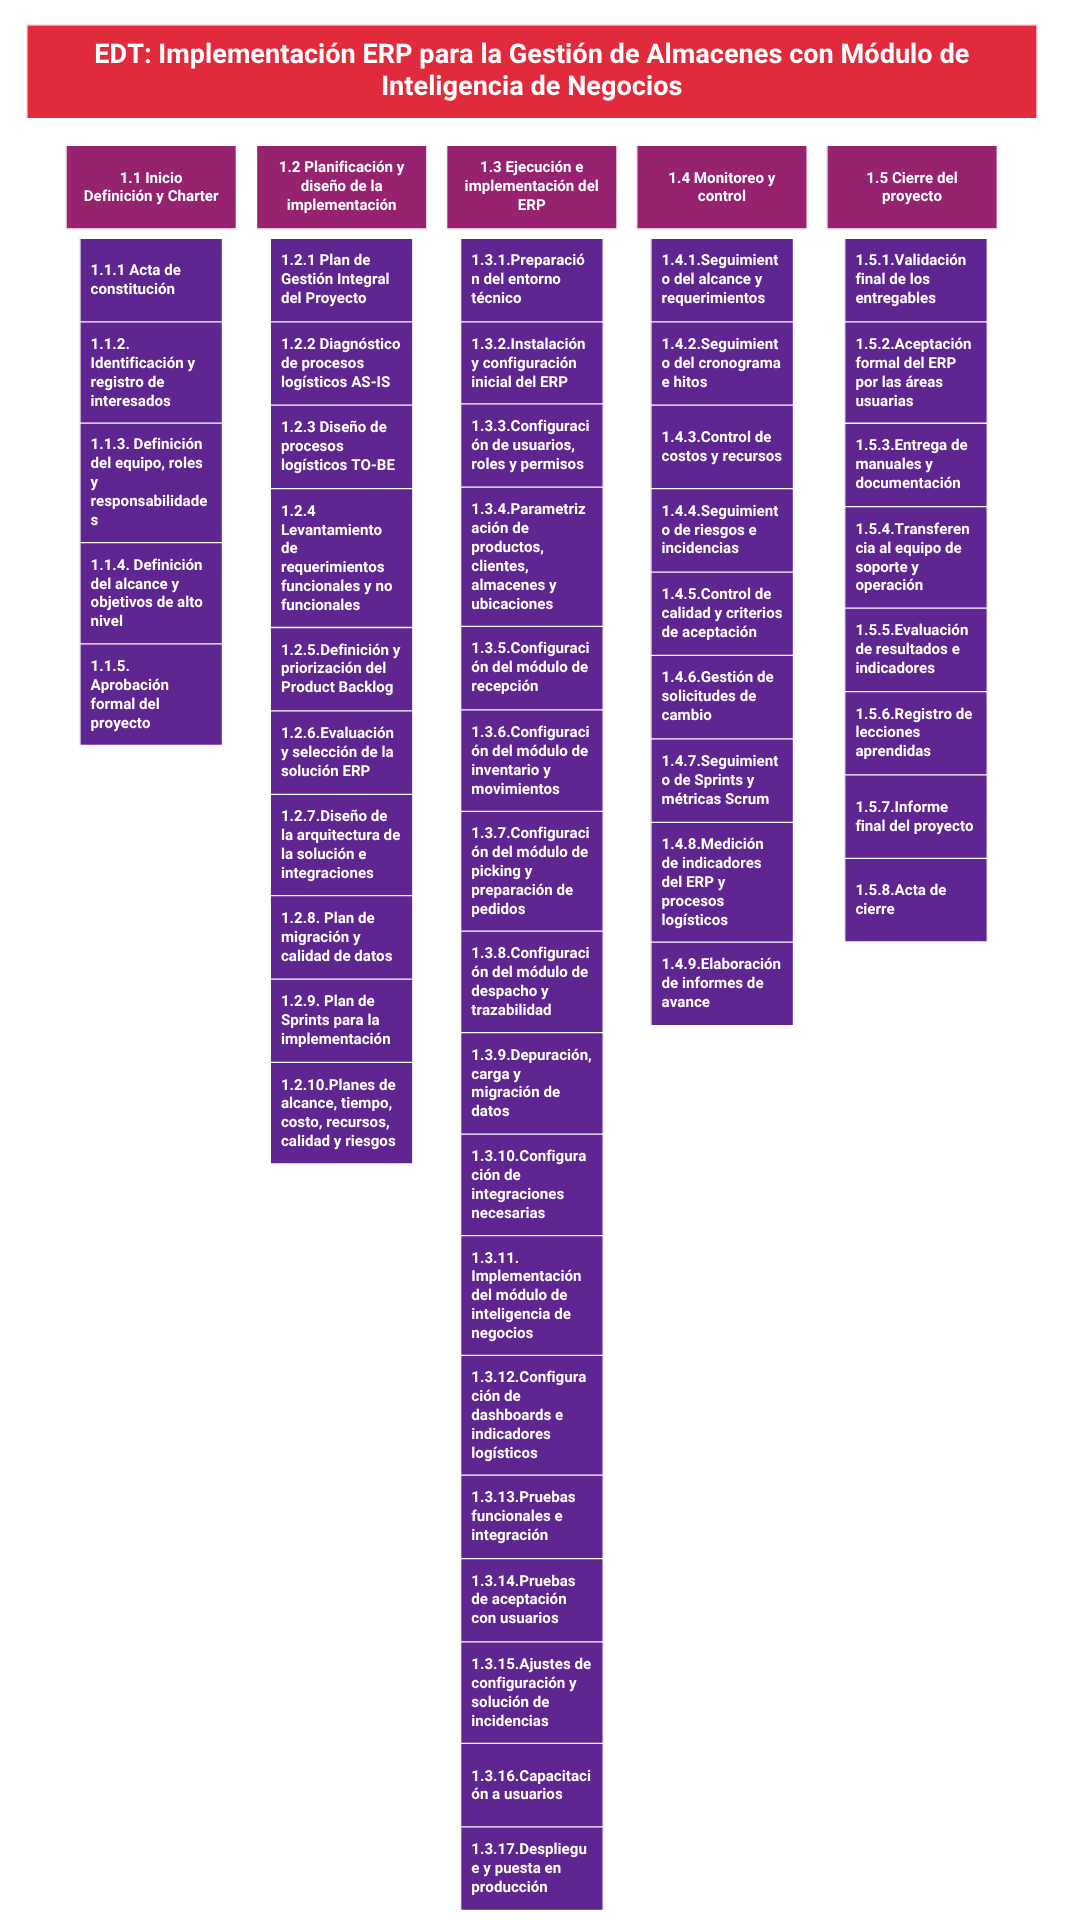
\includegraphics[width=0.9\textwidth]{img/EDT.png}
\end{center}

\section{Cronograma}


% ============================================================
% CAPÍTULO 3
% ============================================================
\chapter{Análisis Económico y Viabilidad}


% ============================================================
% CAPÍTULO 4
% ============================================================
\chapter{Plan de Gestión de Riesgos}


% ============================================================
% ANEXOS
% ============================================================

\appendix
\chapter{Anexos}

\section*{Listado de imágenes a subir en la carpeta \texttt{img/}}

Para que el documento compile con las figuras finales, se deben subir las imágenes en formato PNG dentro de la carpeta \texttt{img/} con los siguientes nombres:

\begin{itemize}
  \item \texttt{logo-upeu.png}
  \item \texttt{mapa-procesos-n0.png}
  \item \texttt{foda-ti.png}
  \item \texttt{pestel-ti.png}
  \item \texttt{mapa-estrategico-negocio.png}
  \item \texttt{mapa-estrategico-ti.png}
  \item \texttt{matriz-alineamiento-negocio-ti.png}
  \item \texttt{ishikawa.png}
  \item \texttt{roadmap-tecnologico.png}
\end{itemize}

\section*{Documento complementario}

Se considera como documento complementario el archivo del proyecto WMS:

\begin{center}
\texttt{Proyecto\_WMS\_CO\_LOGISTIC\_SAC.pdf}
\end{center}

\end{document}